\section{نکات پیاده‌سازی پروژه}

پیاده‌سازی پروژه در زبان جاوا انجام گرفت. یکی از نکات مهم و قابل توجه در پیاده‌سازی این پروژه این است که تمام مراحل انجام کار  به طور کاملاً خودکار انجام شود و در هیچ مرحله‌ای نیاز به دخالت عامل خارجی  ندارد بجز پیکربندی اولیه مانند آدرس پایگاه داده. همچنین در تمام مراحل سعی شده است که تمام اصول لازم در طراحی معماری نرم‌افزار به کار گرفته شود و نیازمندی‌های کیفی پروژه نیز مد نظر قرار گیرد. این نیازمندی‌ها شامل موارد زیر است:
\begin{enumerate}
\item 
\واژه{کارایی} : جهت پاسخ به این نیازمندی از پایگاه داده استفاده شده است.
\item
قابلیت نگهداری: این قابلیت از سایرین بیشتر حائز اهمیت است. زیرا پروژه های پروژهشی خود به صورت مستقیم کاربران عمومی ندارند و از این جهت نیازمند کارایی بالا یا رابط گرافیکی کاربر پسند نیستند. استفاده آن‌ها معمولاً در گسترش آن‌ها توسط سایر محققین است که راه را ادامه خواهند داد. 
\begin{itemize}
\item

 برای پاسخ به این نیازمندی اصول مربوط به کدنویسی  در فصل سوم و چهارم کتاب  \cite{martin2009clean} به کار گرفته شده است.
 \item
 از الگوهای نرم افزاری پر کاربرد مانند \نام{اداپتور}{Adaptor}،  \نام{فکتوری}{Factory} و \نام{سینگلتون}{Singelton} استفاده شده است.
 \item
 به منظور جلوگیری از قطعه کد تکراری از وراثت و توابع \واژه{عمومی} استفاده شده است. همینطور عمق وراثت از عدد ۳ بیشتر نشده است زیرا وراثت عمیق از خوانایی کد می‌کاهد و محل اشتباه خواهد بود. 
\end{itemize}
\item
امنیت: از آنجا که پروژه قرار نیست به استفاده ی عموم برسد و کاربران عمل متخاصمانه‌ای انجام نخواهند داد   به نوع خاصی از امنیت  نسبت به انواع متداول دارد.  باید روند توسعه‌ی پروژه دارای امنیت باشد. از این نظر که کدها مفقود نشوند یا در صورت اشتباه در توسعه بتوان پروژه را به حالت قبل بازگرداند. در این راستا کدهای پروژه در مخزن نرم افزاری از نوع گیت نگهداری شده که یک مخزن در کامپیوتر شخصی و دیگری در سایت \نام{بیت‌باکت}{Bitbucket - \url{https://bitbucket.org/alimohebbi/bug_predict }} 
قرار دارد. مزیت این سایت نسبت به گیت‌هاب این است مخازن خصوصی  را به صورت رایگان ارائه می دهد. در مخازن خصوصی  اجازه‌ی دسترسی تنها به  افراد تعیین شده از طرف مالک  داده می‌شود و عموم کاربران به آن دسترسی ندارند. از ابتدای شروع پیاده‌سازی کدها در مخازن بروزرسانی شده است. نمایی از ثبت‌های مختلف پروژه در مخزن در شکل \ref{fig:bitbucket}
آورده شده است. 
\end{enumerate}

 \begin{figure}[H]
	\centering
	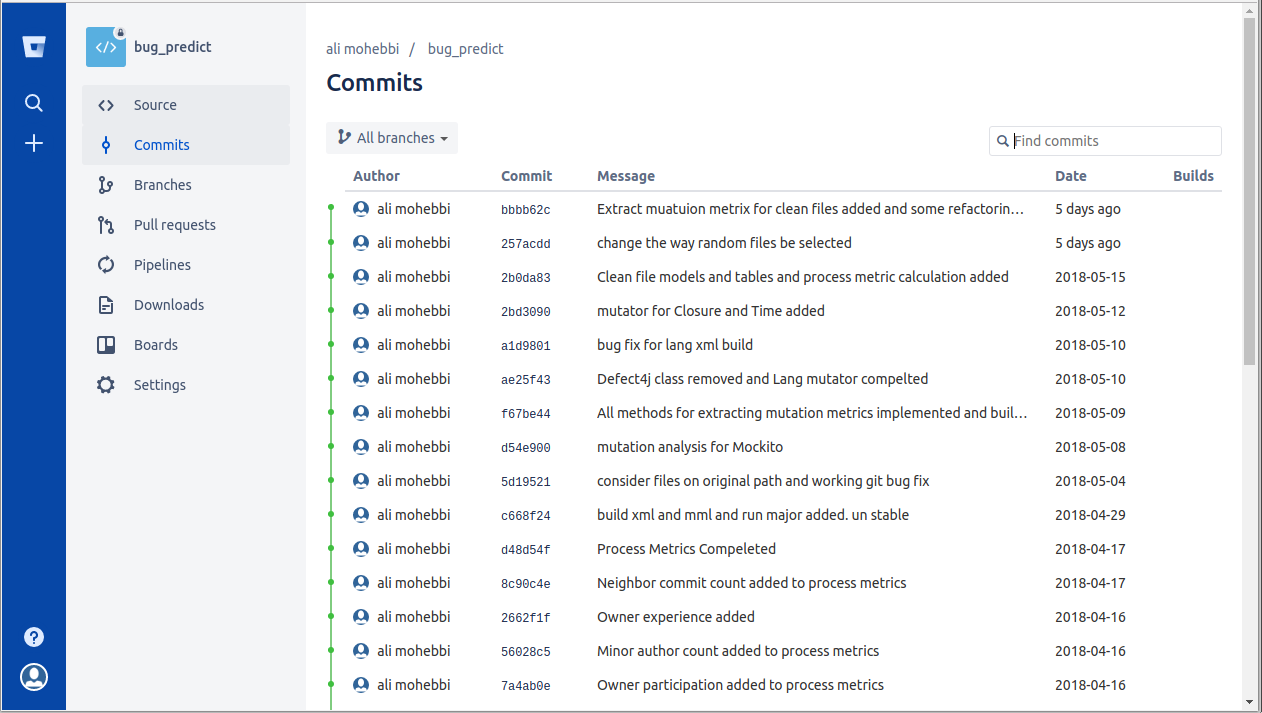
\includegraphics[width=1\textwidth]{img/case_study/bitbucket.png}
	\caption{نمایی از مخزن نرم‌افزاری}
	\label{fig:bitbucket}
\end{figure}


\section{رویکرد اول : معیارهای فرآیند در کنار جهش}

\subsection{ استخراج اطلاعات مربوط به ثبت‌های   حاوی خطا}
اطلاعات مورد نیاز درباره نسخه های حاوی خطا با توجه به معیارهایی که قرار است استخراج شود عبارتند از 
- شماره ی نسخه 
- نام فایل حاوی خطا
- شماره ی خطا در ابزار d4j
- شماره ی نسخه تعمیر خطا
- نام پروژه
- نام انتشار(Release) قبلی پروژه
- شماره ی نسخه ی انتشار قبلی پروژه
از میان اطلاعات بالا همگی به سادگی با استفاده از ابزار defect4j قابل استخراج است بجز دو مورد آخر. همچنین شماره نسخه­ی تعمیر مورد استفاده قرار نگرفت ولی نگهداری شد چراکه ممکن بود لازم شود. در ابتدا محل ذخیره اطلاعات defect4j  به علت تعدد فایلهای مربوط به ابزار و نبود مستندات مشخص نبود. برای استخراج اطلاعات کد ابزار d4j تغییر داده شده تا اطلاعات را علاوه بر خروجی در یک فایل نیز ذخیره کند و سپس در پروژه اطلاعات از فایل خوانده می شد. زبانی که ابزار defect4j با آن نوشته شده perl می‌باشد که یک زبان interpretive است و در آن زمان از اجرای پروژه هنوز IDE‌ مناسبی برای کار کردن با کد های perl پیدا نشده بود. این روش چندان اصولی نیست. با‌گذشت زمان و آشنایی بیشتر با ساختار defect4j محل ذخیره فایلها پیدا شد و از آن پس مستقیماً از فایلها اطلاعات دریافت شد. در d4j اطلاعات خطاها برای هر پروژه به طور جداگانه در یک فایل متنی قرار داده شده بود. 
برای بدست آوردن اطلاعات مربوط به هر انتشار لازم است که مخرن نرم افزاری هر پروژه مورد بررسی قرار گیرد و همچنین آشنایی کافی با مفاهیم پیشرفته git بدست آید. پس از بدست آوردن اطلاعات نتیجه این شد که در پروژه های نرم افزاری برای مشخص کردن یک رویداد مهم از tag استفاده می شود. هر تگ می‌تواند به یک نسخه از برنامه اشاره کند. Tag می‌تواند نمایانگر رویدادهایی چون انتشار برنامه، انتشار بتا، و یا کاندید انتشار باشد. پس با استفاده از تگ می‌تواند انتشار را پیدا کرد.
در قدم اول باید تگ هایی که مربوط به انتشار نیستند جدا شوند. اینکار با استفاده از بررسی نام آنها صورت می گیرد. در صورتی که نام آن‌ها حاوی لغات D4j، RC، Dev یا Strus باشند حذف می شوند. (این لغات با مشاهده ی لیست تگ ها برای پروژهای مختلف بدست آمده). 
در قدم بعدی باید مشخص شود اولین تگ انتشار ما قبل هر نسخه ی حاوی خطا کدام است. 
سه راه حل برای  این مساله ارايه شد که هریک به نوعی با بن‌بست مواجه شدند.  در نهایت جواب نهایی پس از یک هفته پیدا شد. از پرداختن به جزییات پیاده‌سازی در اینجا صرف نظر می شود. در نهایت جدولی به شکل زیر به نام BugInfo تولید شد.
این جدول ۴۰۵ سطر دارد که بیشتر از تعداد کل خطاهای ذکر شده در d4j است. علت این است که در d4j یک خطا می‌تواند خطا در چندین فایل به طور همزمان باشد اما از آنجا که پیش‌بینی در سطح فایل انجام می‌شود لازم است اطلاعات بر اساس فایل‌ها ذخیره شود. همچنین خطاهای موجود در پروژه ی jfreechart در این جدول نیامده است زیرا مشخص شد که پروژه ی jfreechart در مخزنی از نوع git نیست و نوع آن svn‌ است. راهی برای تبدیل آن به git پیدا شد و کنار گذاشته شد تا در زمانی مناسب به git تبدیل شود. البته مشخص شد ساختار این پروژه علی‌رغم تبدیل به git همچنان برای بکارگیری مناسب نیست و راه حلی پیدا نشد. در قسمت مربوطه بیشتر توضیح داده خواهد شد. 

\begin{figure}[H]
\centering
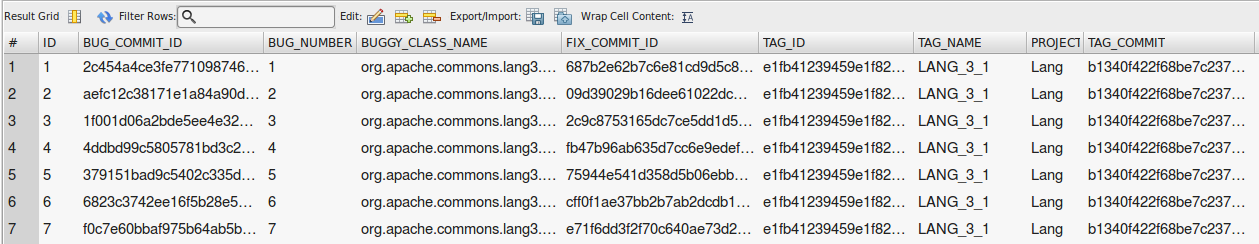
\includegraphics[width=1\textwidth]{img/case_study/bug-info.png}
\caption{نمایی از مخزن نرم‌افزاری}
\label{fig:bug-info}
\end{figure}


\subsection{ استخراج معیارهای فرآیند}

COMM: تعداد نسخه هایی که در آن فایل مورد نظر در طول یک انتشار تغییر کرده است. برای محاسبه ی آن لازم است که تمام نسخه های پروژه بین نسخه ی کنونی و انتشار قبلی بررسی شود و نسخه هایی که در آن این فایل تغییر کرده‌اند شمرده شوند. اولین راه حلی که به ذهن می‌رسد استفاده ی مستقیم از jgit برای این کار است. مشکل این راه این است که بسیار هزینه بر خواهد بود زیرا مرتبا باید عملیات IO بر روی دیسک انجام پذیرد و همچنین بررسی های تکراری بسیاری انجام می گیرد. به عنوان مثال دو نسخه ی حاوی خطا را در نظر بگیرید که دارای انتشار ما قبل یکسانی هستند. تعدادی از بررسی های نسخه های ما بین آن‌ها تا نسخه ی انتشار دارای همپوشانی خواهد بود. از طرف دیگر می‌توان اطلاعاتی که در بررسی نسخه ها بدست می‌آید در محاسبه ی معیارهای دیگر نیز مورد استفاده قرار گیرد. بنابرین کل نسخه های پروژه ها مورد بررسی قرار گرفت و دو جدول تولید شد. 
جدول اول به نام CommitInfo‌ که اطلاعات کلی نسخه ها را در بر می‌گیرد و جدول دوم  CommitChangedFile که اطلاعات مربوط به فایلهایی که در یک نسخه از برنامه نسبت به نسخه ی قبل تغییر کرده است نگهداری می شود. در جدول اول SequenceNumber نشان می‌دهد که چندمین نسخه از ابتدای پروژه می‌باشد و این عدد را خودمان در هنگام بررسی ها به آن نسخه داده‌ایم زیرا برای یافتن نسخه های بین نسخه ی کنونی و نسخه ی انتشار قبلی لازم می‌شود. شاید به ذهن بیاید که از تاریخ هم می‌شد استفاده کرد ولی مشکل اینجا بود که تعداد زیادی از نسخه های ابتدای پروژه دارای تاریخ یکسانی بودند و استفاده از تاریخ غیر ممکن می شد. علت داشتن تاریخ یکسان احتمالاً مهاجرت از یک نوع مخرن نرم افزاری به نوع git بوده است.   هر سطر از جدول دوم یک کلید خارجی دارد به سطری از جدول اول. قسمتی از جداول تولید شده در شکل‌های  زیر آمده است:

\begin{figure}[H]
	\centering
	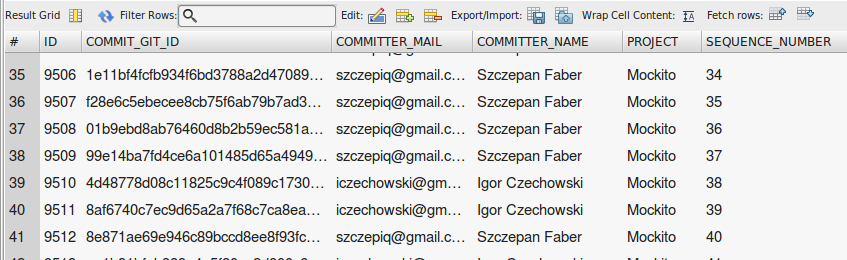
\includegraphics[width=1\textwidth]{img/case_study/commit-info.png}
	\caption{نمایی از مخزن نرم‌افزاری}
	\label{fig:commit-info}
\end{figure}


\begin{figure}[H]
	\centering
	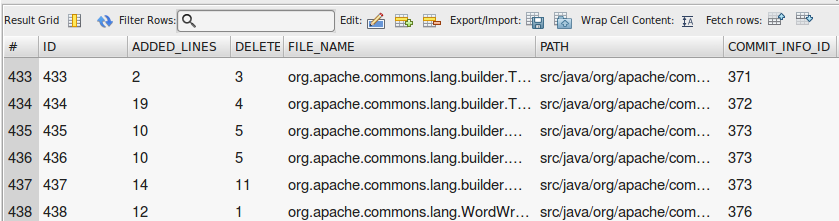
\includegraphics[width=1\textwidth]{img/case_study/change-file-info.png}
	\caption{نمایی از مخزن نرم‌افزاری}
	\label{fig:change-file-info}
\end{figure}

\begin{latin}
\begin{lstlisting}[language=SQL]
SELECT  count(*) from CommitInfo CI where 
CI.SEQUENCE_NUMBER BETWEEN :startSeq AND :endSeq 
AND CI.PROJECT = :project AND CI.COMMITTER_MAIL = :authorEmail

\end{lstlisting}
\end{latin}
\captionof{lstlisting}{سیا}